\documentclass[12pt]{article}
\usepackage{amsmath}
\usepackage{amsfonts}
\usepackage{graphicx}

\begin{document}

\section*{Question 4}

The variable \( X \) represents the number of cigarettes sold per year (in hundreds per capita), and the variable \( Y \) represents the number of lung cancer deaths per 10,000 inhabitants in 1960. The following data points are observed.

\subsection*{1.}

Let the number of samples be:
\[
n = 11
\]

Let the values of \( X \) in ascending order be:
\[
X_1 = 18.20, \, X_2 = 18.24, \, \dots, \, X_i, \, \dots, \, X_n = 40.46, \quad i \in \{1, 2, \dots, n\}
\]

As well as the corresponding values of \( Y \):
\[
Y_1 = 17.05, \, Y_2 = 15.98, \, \dots, \, Y_i, \, \dots, \, Y_n = 27.27, \quad i \in \{1, 2, \dots, n\}
\]

Then, we have the mean of \( X \) and the mean of \( Y \) as:
\[
\bar{X} = \frac{1}{n} \sum_{i=1}^n X_i = \frac{29,848}{1,100} \approx 27.135
\]
\[
\bar{Y} = \frac{1}{n} \sum_{i=1}^n Y_i = \frac{2,298}{110} \approx 20.891
\]

Then, we compute the covariance of \( X \) and \( Y \):
\[
\sigma_{XY} = \frac{1}{n} \sum_{i=1}^n X_i Y_i - \bar{X} \bar{Y} \approx 23.093 > 0
\]

Hence, we can conclude that \( Y \) increases with respect to \( X \).

\textbf{Answer:} Increasing

\subsection*{2.}

Assume that \( Y \) approximately grows linearly with respect to \( X \):
\[
Y_i \approx a X_i + b, \quad i \in \{1, 2, \dots, n\}
\]

Let the variance of \( X \) (denoted \( \sigma_X^2 \)) be:
\[
\sigma_X^2 = \frac{1}{n} \sum_{i=1}^n X_i^2 - \bar{X}^2 \approx 40.927
\]

Then, we calculate \( a \) as:
\[
a = \frac{\sigma_{XY}}{\sigma_X^2} \approx 0.564
\]

Next, we calculate \( b \) as:
\[
b = \bar{Y} - \frac{\sigma_{XY}}{\sigma_X^2} \bar{X} = \bar{Y} - a \bar{X} \approx 5.580
\]

Thus, the linear relationship between \( Y \) and \( X \) is given by:
\[
Y_i \approx 0.564 X_i + 5.580, \quad i \in \{1, 2, \dots, 11\}
\]

\textbf{Answer:}
\[
Y_i \approx 0.564 X_i + 5.580, \quad i \in \{1, 2, \dots, 11\}
\]

\begin{figure}[h!]
\centering
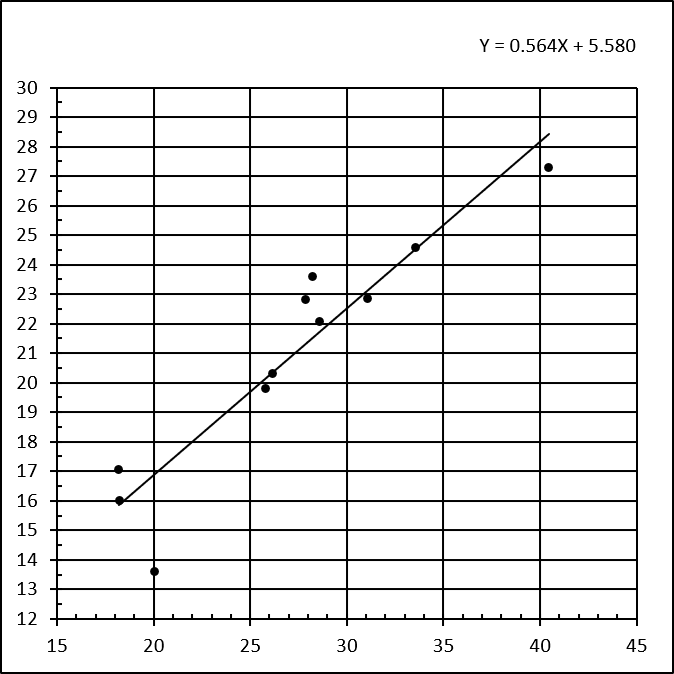
\includegraphics[width=0.5\textwidth]{Q4-P2-graph.png}
\caption{Graph of the relationship between \( Y \) and \( X \)}
\end{figure}

\end{document}
